%\begin{filecontents*}{example.eps}
%!PS-Adobe-3.0 EPSF-3.0
%%BoundingBox: 19 19 221 221
%%CreationDate: Mon Sep 29 1997
%%Creator: programmed by hand (JK)
%%EndComments

%\end{filecontents*}
%
%\documentclass{svjour3}                     % onecolumn (standard format)
%\documentclass[smallcondensed]{svjour3}     % onecolumn (ditto)
\documentclass[12pt,oneside,a4paper]{article}  

\usepackage{apacite}
\usepackage{appendix}
\usepackage{amsmath}
\usepackage{amsthm}
% for ASY interactive 3d figure
\usepackage[inline]{asymptote}
\usepackage{amssymb} % for approx greater than
\usepackage{caption}
\usepackage{placeins} % for \FloatBarrier
\usepackage{graphicx}
%\usepackage{subcaption}
\usepackage{longtable}
\usepackage{setspace}
\usepackage{booktabs}
\usepackage{tabularx}
\usepackage{xcolor,colortbl}
\usepackage{chngpage}
\usepackage{natbib}
\bibpunct{(}{)}{,}{a}{}{;} 
\usepackage{url}
\usepackage{nth}
\usepackage{authblk}
\usepackage[most]{tcolorbox}
\usepackage[normalem]{ulem}
\usepackage{amsfonts}

% columns for longtable
%\usepackage{arydshln} % Dashed lines in matrices

\usepackage[margin=1in]{geometry}
%\doublespacing % for review

% line numbers to make review easier
%\usepackage{lineno}
%\linenumbers

%\usepackage{soul}% for \st{}

%%%%%%%%%%%%%%%%%%%%%%%%%%%%%%%%%%%%%%%%%%%%%%%%%%%%%%%%%%%%%%%%%%%%%%%%%%%%%%
% for section 4 math environments
%\theoremstyle{definition}
%\newtheorem{definition}{Definition}[section]
%\newtheorem{theorem}{Theorem}[section]
%\newtheorem{proposition}{Proposition}[section]
%\newtheorem{corollary}{Corollary}[proposition]
%\newtheorem{remark}{Remark}[section]
%
%%%%%%%%%%%%%%%%%%%%%%%%%%%%%%%%%%%%%%%%%%%%%%%%%%%%%%%%%%%%%%%%%%%%%%%%%%%%%%
%\begin{filecontents*}{example.eps}
%!PS-Adobe-3.0 EPSF-3.0
%%BoundingBox: 19 19 221 221
%%CreationDate: Mon Sep 29 1997
%%Creator: programmed by hand (JK)
%%EndComments
%gsave
%newpath
%  20 20 moveto
%  20 220 lineto
%  220 220 lineto
%  220 20 lineto
%closepath
%2 setlinewidth
%gsave
%  .4 setgray fill
%grestore
%stroke
%grestore
%\end{filecontents*}
%\RequirePackage{fix-cm}

\newcommand\ackn[1]{%
  \begingroup
  \renewcommand\thefootnote{}\footnote{#1}%
  \addtocounter{footnote}{-1}%
  \endgroup
}

% Affiliations in small font size
%\renewcommand\Affilfont{\small}
\newcommand{\absdiv}[1]{%
  \par\addvspace{.5\baselineskip}% adjust to suit
  \noindent\textbf{#1}\quad\ignorespaces
}

%\defcitealias{HMD}{HMD 2016}

% junk for longtable caption
%\AtBeginEnvironment{longtable}{\linespread{1}\selectfont}
%\setlength{\LTcapwidth}{\linewidth}

% sort van Raalte properly
% #1: sorting key, #2: prefix for citation, #3: prefix for bibliography
%\DeclareRobustCommand{\VAN}[3]{#2} % set up for citation
%\newcommand{\tc}{\quad\quad\text{,}}
%\newcommand{\tp}{\quad\quad\text{.}}
%%%%%%%%%%%%%%%%%%%%%%%%%%%%%%%
\begin{document}


\title{A note on independant time measures}

%\author{Tim Riffe \and Neil Mehta \and Daniel Schneider \and Mikko Myrskyl\"a}
\author[1]{Tim Riffe\thanks{riffe@demogr.mpg.de}}
\author[2]{Joel Cohen}


\affil[1]{Max-Planck-Institute for Demographic Research}
\affil[2]{The Rockefeller University}


%\authorrunning{Short form of author list} % if too long for running head

\maketitle

\vspace{-2em}
\begin{abstract}
\absdiv{Background} There are countless Lexis-like relationships between
linearly dependant time measures, and these can be combined into higher-order
Lexis identities with dense linear dependencies. One such relationship is the demographic time identity between age, period, cohort, time to death,
length of life, and time of death. Certain subsets of time measures in this
and other higher order identities consist in time measures that are independant
of one another.
\absdiv{Objective} We aim to describe the relationship between
independent time measures and the identities within which they are nested, with
special attention to the demographic time identity and its three independant
time dyads. We aim to determine whether data structured on such time dyads might
be useful in demographic research.
\absdiv{Data and Methods} We illustrate concepts visually based on data from the
Colonial Qu\'{e}bec Population Register.
\absdiv{Results}
\absdiv{Conclusions}
\end{abstract}

\section{Geometric relationships}
The demographic time identity maps to the edges of a tetrahedron. When extended
into three dimensions, the tedtrahedron tesselates with octahedra in a 2:1
ratio. In its original description \citep{riffe2017demographictime}, neither
independant pairs of time measures nor the significance of octahedra in this
geometric construct were considered in any depth. Figure~\ref{fig:tet}
shows the tetragedral graph of the demographic time identity between age
(A), period (P), cohort (C), time to death (T), death cohort (D), and length
of life (L). Independant dyads are those that do not share any vertex in the
graph, and these appear already as perpendicular in the present graph
representation: CT, LP, and AD.

\begin{figure}[h!]
\centering
\caption{Tetrahedral graph of demographic time hexad identity, with edges
labelled by the six time indices. Reproduced from 
\citet{riffe2017demographictime}.}
\label{fig:tet}
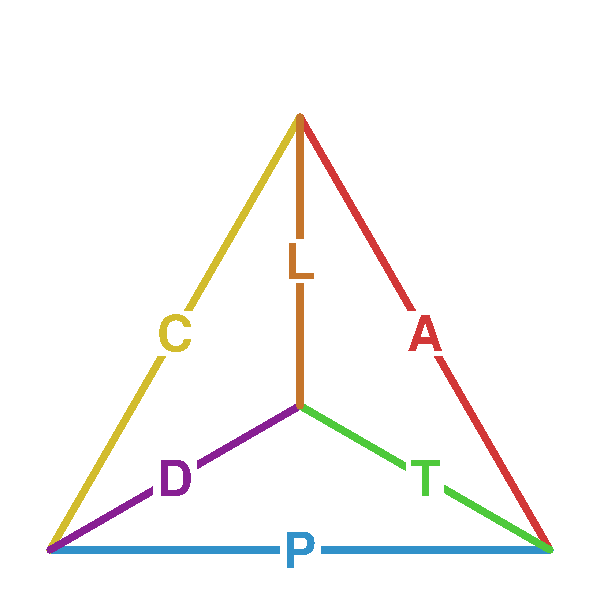
\includegraphics[width=4in]{Figures/TetraHedronEdgesOnly.pdf}%
\end{figure}

Pairs of independant dyads can be extended onto a Cartesian plane, which is
already an isometric projection, and these planes can also represent
cross-sections of a 3d demographic time space. The independant planes can also
be conceived of a angles of view on the demographic time space. 

\subsection{Angles of view}
An angle of view directly at any of the four faces of the demographic
time tetrahedron reveals the plane-perspective defined by one of the
Lexis-like identities.\footnote{In other words, set the viewing axis as
\emph{normal} to one of the faces of the plane.} Independant dyad planes are
revealed when the viewing angle is such that the midpoints of opposite
tetrahedral edges are aligned. There are three pairs of
opposite edges (LP, TC, AD), and therefore three viewing angles of this kind.
This turns out to being identical to the angle required to directly view a face of the cube-dual of an octahedron in the same structure tetrahedral-octahedral structure. The cube dual
is also a space-filling tesselation, with each of its eight vertices
forming the centroid of a tetrahedron. It is for our
purposes therefore spatially redundant with the tetrahedral-octahedral
honeycomb.

\begin{figure}
\input{tetratex.tex}
\end{figure}



% bibliography
\bibliographystyle{chicago}
\bibliography{references}  
\end{document}

